\chapter{Software}

\section{HTML5}
\cite{w3schools_html}
\section*{Erläuterung}
HTML5 ist die fünfte Generation der Hypertext Markup Language. HTML wird hauptsächlich zur Darstellung von Websites im Internet genutzt. Die HTML-Dateien werden dabei von einem Browser abgerufen und dargestellt. Die Auszeichnungssprache wird vom World Wide Web Consotrium (W3C) laufend weiterentwickelt. Die 5. Version ist das erste Mal 2008 publiziert worden.

\section*{Funktionalität}
Dadurch das HTML mit CSS und JavaScript um ein Design und Funktionen erweitert werden kann, ist es sehr flexibel und vielseitig einsetzbar. Ganze Programme werden heute als WebApp programmiert und bieten denselben Funktionsumfang wie herkömmliche desktopbasierte Programme. Weil nur ein Browser benötigt wird, um die Websites darzustellen sind, sie außerdem plattformunabhängig.


\section*{Verwendung}
HTML bildet das Fundament für den Bad-Designer, auf dem alle anderen Features aufbauen. Die Modelle der sanitären Anlagen werden hier geladen. Die restlichen Funktionen werden mit JavaScript [\ref{sec:JavaScript}] implementiert.

\newpage
\clearpage

\section{JavaScript}\label{sec:JavaScript}
\cite{wiki_js}


\section*{Erläuterung}
JavaScript ist eine Skriptsprache, die dazu dient, HTML zu erweitern. Damit kann man auf Benutzerinteraktionen reagieren und diese auswerten, Inhalte verändern, generieren und nachladen. Somit sind die Seiten dynamisch und ergänzen HTML und CSS so dass sie interaktiv werden. Des Weiteren wird JavaScript auch für Server und Microcontroller verwendet. Eine bekannte serverseitige Plattform, nämlich Node.js, basiert auf der JavaScript-Laufzeitumgebung. 
\\
Die Syntax der 1995 erschienenen Sprache ähnelt der von C. Obwohl Java auf Gemeinsamkeiten vermuten lässt ist JavaScript deutlich anders und vieles abweichend implementiert. Durch die Variabilität ist es möglich objektorientiert, prozedural oder funktional zu programmieren.

\section*{Funktionalität}
JavaScript bildet mit seinen umfangreichen Funktionen das Grundgerüst für die Diplomarbeit. Animationen, Berechnungen, Benutzer Interaktionen und Datenverarbeitung werden es dadurch möglich.


\section*{Verwendung}
Das Laden der Modelle, Animationen, Benutzer Eingaben und Berechnungen wurden allesamt in JavaScript realisiert. JavaScript ist der wichtigste Bestandteil der Arbeit, die meisten Funktionen wären ohne diese Skriptsprache nicht möglich.  Außerdem basiert die Bibliothek three.js [\ref{sec:three.js}] auf dieser Sprache und erweitert sie. Mehr zu three.js wird auf den folgenden Seiten näher erläutert.

\newpage
\clearpage


\section{WebGL}\label{sec:WebGL}
\cite{khronos_webgl}\cite{mdn_webgl}
\section*{Erläuterung}
WebGL, kurz für Web Graphics Library, ist eine auf JavaScript basierende Programmierschnittstelle, die es ermöglicht 3D-Grafiken hardwarebeschleunigt im Webbrowser ohne zusätzliche Erweiterungen, Bibliotheken und Technologien darzustellen. Des Weiteren basiert WebGL auf den Spezifikationen von OpenGL ES, kurz für Open Graphics Library for Embedded Systems. Diese beschreibt eine plattform- und sprachenunabhängige Programmierschnittstelle für die Entwicklung von 3D-Computergrafiken. 
\\
Die 2011 erschienene Library ist lizenzfrei von der Khronos Group und Mozilla entwickelt worden. Mit der Zeit haben immer mehr Unternehmen die Entwicklung unterstützt, dazu zählen unteranderem Google Chrome, AMD, Ericsson, Nvidia und Opera. 


\section*{Funktionalität}
Dadurch, dass die Grafik-Bibliothek im Browser läuft, ist sie plattformunabhängig und hat unteranderem deshalb auch eine große Reichweite. \\Zusätzlich gestattet sie Grafikern mit den beliebten Softwarewerkzeugen wie Blender, Maya oder CopperCube zu arbeiten ohne sich um die Darstellung anschließend kümmern zu müssen. WebGL konfiguriert und verarbeitet die Modelle für den Browser.

\section*{Verwendung}
WebGL kann für eine Vielzahl von Dingen verwendet werden, durch immer leistungsfähigere Geräte und Anwendungen wird das Anwendungsgebiet größer. Hauptsächlich wird es für 3D Modelle im Internet genutzt. Vor allem im Marketing Bereich wird die Anwendung kontinuierlich beliebter, da die Hersteller nun die Möglichkeit haben, dem Kunden das Produkt auf einem zwei dimensionalen Bildschirm drei dimensional darzustellen. Dadurch steigt die Verkaufswahrscheinlichkeit wesentlich an, da der Kunde eine Übersicht bekommt als hätte er sich das Produkt in echt angesehen.
\\
Das Laden der Badezimmer-Module übernimmt WebGL und dient gleichzeitig als Basis für three.js. Die ganzen Animationen und Effekte werden von dieser Bibliothek abgewickelt.



\newpage
\clearpage


\section{three.js} \label{sec:three.js}
\cite{Three.js_GitHub} \cite{Three.js}
\section*{Erläuterung}
three.js ist eine browserübergreifende JavaScript [\ref{sec:JavaScript}]  Bibliothek und API mit der im Browser dreidimensionale Objekte kreiert und angezeigt werden können. Die Besonderheit ist dabei dass three.js auf WebGL [\ref{sec:WebGL}] basiert, dadurch werden Inhalte über die Grafikkarte gerendert was wiederum zu mehr Performance und kürzere Ladezeiten führt. Die Bibliothek ist das erste Mal im April 2010 unter der MIT-Lizenz [\ref{sec:MIT}] erschienen und wird in einem Repository auf GitHub [\ref{sec:Git}] gehostet.

\section*{Funktionalität}
Dadurch dass die Library in JavaScript [\ref{sec:JavaScript}]   geschrieben wurde und auf WebGL [\ref{sec:WebGL}] aufsetzt ist die Interoperabilität zwischen den verschiedensten Browsern und Betriebssystemen gewährleistet, ohne zusätzliche proprietäre Plug-Ins zu verwenden. Außerdem unterstützt sie auch Virtuelle Realität und vieles mehr.

\section*{Verwendung}
Alle Module des Badezimmers werden per three.js geladen und animiert. Jegliche Animationen, Effekte und Texturen werden erst durch diese Technologie möglich. Die Bibliothek ist verantwortlich für die meisten Vorgänge im Bad-Designer und ist somit der wichtigste Bestandteil des Projektes.

\newpage
\clearpage

\section*{Struktur}
\cite{Fundamentals_English}
\cite{Fundamentals_German}
\begin{figure}[h]
    \centering
    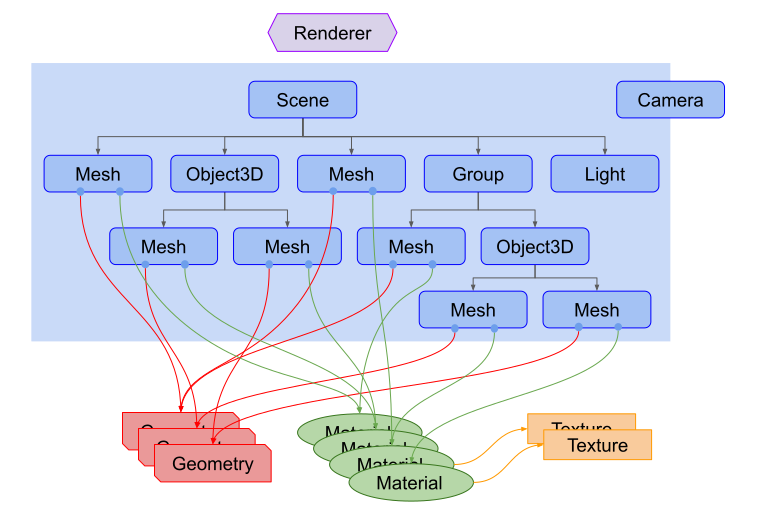
\includegraphics[width=0.9\textwidth]{images/threejs-structure.png}
    \caption{Die Struktur von three.js \cite{threejs_structure}}
    \label{fig:my_label}
\end{figure}

\subsection{Canvas}
In HTML5 ist der Canvas ein Element das dafür benutzt wird, Grafiken, Pfade, Texte und Bilder darzustellen. Ein Canvas kann animiert werden, außerdem reagiert er auf JavaScript-Events beziehungsweise auf Benutzereingaben wie Mausklicks oder Mausbewegung. Dieses Objekt wird von allen gängigen Browsern unterstützt und bietet so three.js eine beständige Grundlage, Grafiken im Web darzustellen. \cite{w3canvas}
\\
HTML:
\begin{lstlisting}
<canvas id="canvas" canvas>
\end{lstlisting}
\newpage
\subsection{Renderer}
Der Renderer in three.js ist das Hauptelement dieser Technologie. Ihm wird eine Szene und eine Kamera übergeben, und dann werden die Elemente der 3D-Szene die im Kegelstumpf, auch genannt Blickfeld der Kamera liegen auf einen Canvas (Leinwand) gezeichnet.\\
JavaScript Initialisierung:
\begin{lstlisting}
renderer = new THREE.WebGLRenderer();
renderer.setSize(window.innerWidth, window.innerHeight)
document.getElementById("canvas").appendChild(renderer.domElement);
renderer.render(scene, camera);
\end{lstlisting}
Dem WebGLRenderer wird eine Größe übergeben, anschließend wird er dem in HTML erstellten Canvas, beigelegt. Durch Aufruf der Funktion „render()“ beginnt der Renderer die Szene zu zeichnen.
\subsection{Szene}
Der Szene werden nun alle Objekte, denen deren Position, Orientierung und Materialien hinterlegt wurden, hinzugefügt. Um dem Canvas Daten liefern zu können, muss außerdem eine Kamera beifügt werden. Um Schatten und realistischere Darstellungen zu gewährleisten werden gegebenenfalls Lichtquellen erstellt und hinzugefügt. 
\cite{Szenengraph}
\\
JavaScript Initialisierung:
\begin{lstlisting}
var scene = new THREE.Scene();
\end{lstlisting}
\textbf{Elemente zur Szene hinzufügen:}\\
Alle Objekte die von three.js dargestellt werden sollen, müssen der Szene angehängt werden. Dadurch kann der Renderer auf Änderungen reagieren und neue Darstellungen zeichnen.
JavaScript Funktionalität:
\begin{lstlisting}
scene.add( cube );
\end{lstlisting}
\textbf{Die Szene rendern:}\\
Um Animationen und komplexere Darstellungen zu realisieren ist eine Animations-Schleife notwendig. Dieser Code kann individuell geändert werden um das Programm ressourcenschonender und reaktiver zu machen.\\
JavaScript Funktionalität: 
\begin{lstlisting}
function animate() {
    requestAnimationFrame( animate );
    renderer.render( scene, camera );
}
animate();
\end{lstlisting}
Diese Programmcode kreiert eine Schleife die den Renderer befiehlt, jedes mal wenn der Bildschirm neu geladen wird, die Szene neu zu zeichnen. Bei einem gängigen Computermonitor würde das bedeuten das die Szene 60 mal in der Sekunde neu gerendert wird. \\
Die Funktion requestAnimationFrame() bietet einige Vorteile gegenüber dem konventionellem setInterval(). \\
Der wichtigste Vorteil neben dem dass die Bildwiederholrate optimiert und Browser-Optimierungen vorgenommen werden, ist dass die Schleife pausiert wird, wenn der Benutzer auf ein anderes Web-Browser Fenster wechselt. Dadurch wird nur Prozessorleistung verwendet, wenn sie wirklich vom Programm benötigt wird. \cite{rendering_the_scene}
\\
\\
\textbf{Performance Verbesserungen:}\\
Bei statischen Darstellungen von Objekten mit three.js ist es nicht notwendig die Szene dauerhaft zu rendern. Durch das Hinzufügen von JavaScript Code, kann man die Standardkonfiguration von three.js verändern um das Rendern performanter zu machen.
\\
JavaScript Funktionalität: 
\begin{lstlisting}
function shouldRender() {
    if (needsUpdate) {
        needsUpdate = false;
        return true;
    } else {
        return false;
    }
}

function animate() {
    setTimeout(function () {
        requestAnimationFrame(animate);
    }, 50);
    render();
};

function render() {
    if (shouldRender()) {
        renderer.render(scene, camera);
    }
}
\end{lstlisting}
Die Funktion shouldRender() bietet dem Programmierer die Möglichkeit, abhängig von einer booleschen Variable, die Szene zu rendern, die Funktion requestAnimationFrame() wird mit einer Latenz aufgerufen. \\
Außerdem können auch Event-Listeners auf Benutzereingaben reagieren und die Szene bei diesen Aktivitäten zu rendern. \cite{rendering_on_demand}

\clearpage
\subsection{Geometrie}
Three.js bietet 42 unterschiedliche, vorkonfigurierte Formen die mit wenigen Code-Zeilen einem Objekt hinzugefügt werden können. Diese werden auch als \textit{primitive Geometrien} betitelt. \\
\\
\textbf{Arten:}  \cite{geometry_types} \\
\begin{itemize}
    \item BoxBufferGeometry 
  
Die BoxBufferGeometry bietet die Möglichkeit primitive würfel- oder quaderförmige Objekte zu erstellen.

Definition:
\begin{lstlisting}
BoxBufferGeometry(width : Float, height : Float, 
depth : Float, widthSegments : Integer, 
heightSegments : Integer, depthSegments : Integer)
\end{lstlisting}
\begin{figure}[h]
    \begin{subfigure}{0.5\textwidth}
    \centering
    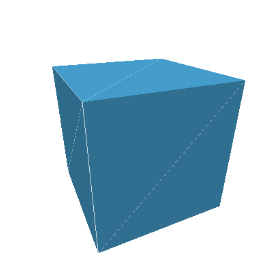
\includegraphics[width=0.5\linewidth]{images/cube.png} 
    \caption{BoxBufferGeometry}
    \label{fig:subim1}
    \end{subfigure}
    \begin{subfigure}{0.5\textwidth}
    \centering
    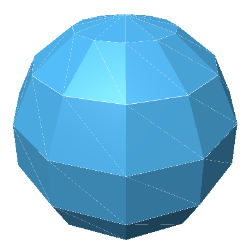
\includegraphics[width=0.5\linewidth]{images/kugel.png}
    \caption{SphereBufferGeometry}
    \label{fig:subim2}
    \end{subfigure}
\caption{Three.js Primitives: Würfel und Kugel \cite{geometry_types}}
\label{fig:image2}
\end{figure}

\item SphereBufferGeometry 
  
Die SphereBufferGeometry bietet die Möglichkeit kugelförmige Objekte zu erstellen. Mit den Werten \textit{widthSegments} und \textit{heightSegments} kann man die Anzahl der Flächen festlegen aus denen die Kugel zusammengesetzt ist. Ein höherer Wert in diesen Parametern resultiert in eine glatteren Oberfläche der Kugel.

Definition:
\begin{lstlisting}
SphereBufferGeometry(radius : Float, widthSegments : Integer,
heightSegments : Integer, phiStart : Float, phiLength : Float,
thetaStart : Float, thetaLength : Float)
\end{lstlisting}
\newpage
\item EdgesGeometry 
  
Die EdgesGeometry bietet die Möglichkeit, die Kanten eines Objekte zu visualisieren.

Definition:
\begin{lstlisting}
EdgesGeometry( geometry : Geometry, thresholdAngle : Integer )
\end{lstlisting}
\begin{figure}[h]
    \begin{subfigure}{0.5\textwidth}
    \centering
    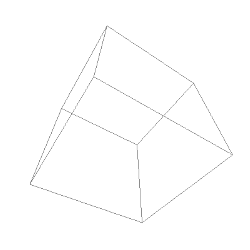
\includegraphics[width=0.5\linewidth]{images/edges.png} 
    \caption{EdgesGeometry}
    \label{fig:subim1}
    \end{subfigure}
    \begin{subfigure}{0.5\textwidth}
    \centering
    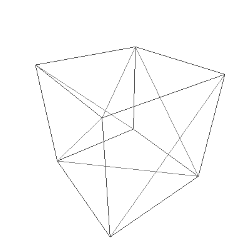
\includegraphics[width=0.5\linewidth]{images/wireframe.png}
    \caption{WireframeGeometry}
    \label{fig:subim2}
    \end{subfigure}
\caption{Three.js Primitives: Kanten und Drahtmodell \cite{geometry_types}}
\label{fig:image2}
\end{figure}

\item WireframeGeometry 
  
Die WireframeGeometry bietet die Möglichkeit Objekte in einem sogenannten \textit{Drahtmodell} darzustellen, um zum Beispiel, Bereiche und Verbindungen besser sichtbar zu machen.

Definition:
\begin{lstlisting}
WireframeGeometry( geometry : Geometry )
\end{lstlisting}

\item PlaneBufferGeometry 
  
Die PlaneBufferGeometry bietet die Möglichkeit Objekte 2D - Flächen zu erstellen.

Definition:
\begin{lstlisting}
PlaneBufferGeometry(width : Float, height : Float,
widthSegments : Integer, heightSegments : Integer)
\end{lstlisting}
\newpage
\begin{figure}[h]
    \begin{subfigure}{0.5\textwidth}
    \centering
    
\includegraphics[width=0.5\linewidth]{images/plane.png} 
    \caption{PlaneBufferGeometry}
    \label{fig:subim1}
    \end{subfigure}
    \begin{subfigure}{0.5\textwidth}
    \centering
    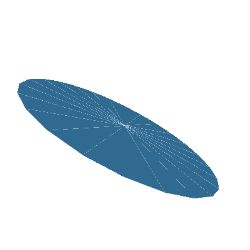
\includegraphics[width=0.5\linewidth]{images/circle.png}
    \caption{CircleBufferGeometry}
    \label{fig:subim2}
    \end{subfigure}
\caption{Three.js Primitives: 2D Flächen und Kreise \cite{geometry_types}}
\label{fig:image2}
\end{figure}

\item CircleBufferGeometry 
  
Die CircleBufferGeometry bietet die Möglichkeit Objekte 2D - Kreise zu erstellen. Mit dem Wert \textit{segments} kann die Anzahl der Dreiecke aus dem der Kreis zusammengesetzt ist festgelegt werden, der minimal Wert ist 3.

Definition:
\begin{lstlisting}
CircleBufferGeometry(radius : Float, segments : Integer,
thetaStart : Float, thetaLength : Float)
\end{lstlisting}

\item ConeBufferGeometry 
  
Die ConeBufferGeometry wird dafür verwendet kegelförmige 3D-Objekte zu erstellen. 
Mit dem booleschen Parameter \textit{openEnded} verändert man ob der Kegel am unteren Ende geschlossen oder offen ist. Der Standardwert ist false, dass bedeutet das der Kegel mit einer extra Fläche bestückt ist.

Definition:
\begin{lstlisting}
ConeBufferGeometry(radius : Float, height : Float,
radialSegments : Integer, heightSegments : Integer,
openEnded : Boolean, thetaStart : Float, thetaLength : Float)
\end{lstlisting}
\newpage

\begin{figure}[h]
    \begin{subfigure}{0.5\textwidth}
    \centering
    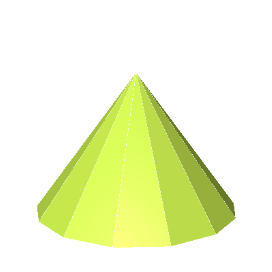
\includegraphics[width=0.5\linewidth]{images/kegel.png} 
    \caption{ConeBufferGeometry}
    \label{fig:subim1}
    \end{subfigure}
    \begin{subfigure}{0.5\textwidth}
    \centering
    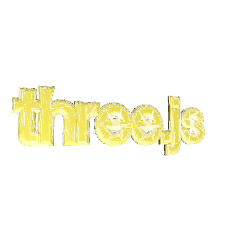
\includegraphics[width=0.5\linewidth]{images/text.png}
    \caption{TextBufferGeometry}
    \label{fig:subim2}
    \end{subfigure}
\caption{Three.js Primitives: 3D Kegel und Text \cite{geometry_types}}
\label{fig:image2}
\end{figure}

\item TextBufferGeometry 
  
Die TextBufferGeometry kann 3D-Texte in einer three.js Szene darstellen. Es gibt Anpassungsmöglichkeiten die dabei helfen den Text zu formatieren.

Definition:
\begin{lstlisting}
TextBufferGeometry(text : String, parameters : Object)
\end{lstlisting}
\textbf{Dem Wert \textit{parameters: Object} können folgende Parameter zugewiesen werden:}
\begin{itemize}
    \item font: Eine Instanz von THREE.Font.
    \item size: Schriftgröße des Texts.\\ Der Standardwert ist 100. (Datentyp: Float)
    \item height: Dicke des Texts.\\ Der Standardwert ist 50. (Datentyp: Float)
    \item curveSegments — Die Anzahl der Punkte auf den Kurven.\\ Der Standardwert ist 12. (Datentyp: Integer)
    \item bevelEnabled — Abschrägungen einschalten.\\ Der Standardwert ist False. (Datentyp: Boolean)
    \item bevelThickness — Wie tief die Abschrägungen in den Text ragen.\\ Der Standardwert ist 10. (Datentyp: Float)
    \item bevelSize — Wie weit die Abschrägung über den Textrand ragt. \\ Der Standardwert ist 8. (Datentyp: Float)
    \item bevelOffset — Float.  Wie weit entfernt die Abschrägung vom Textrand beginnt.\\ Der Standardwert ist 0. (Datentyp: Float)
    \item bevelSegments — Integer. Anzahl der Abschrägungs-Segmente \\ Der Standardwert ist 3. (Datentyp: Integer)
\end{itemize}
\end{itemize}
\newpage
\subsection{Material}
\\ \cite{material} \\
In three.js gibt es 18 unterschiedliche Material-Typen, die einem Objekt zugewiesen werden können. Sie verändern maßgeblich die Darstellung des Objektes und außerdem auch die Reaktion des Elements auf Lichteinstrahlung. Alle Materialien in three.js werden vom Renderer unabhängig erstellt, durch diese Konfiguration müssen Materialien nicht umgeschrieben werden wenn man einen anderen Renderer verwendet. \\
Ein Material ist neben der Geometrie, einer der beiden Hauptbestandteile eines Objektes.
\\ \\
\textbf{Arten:}  \cite{three.js_material} \\
\begin{figure}[h]
    \centering
    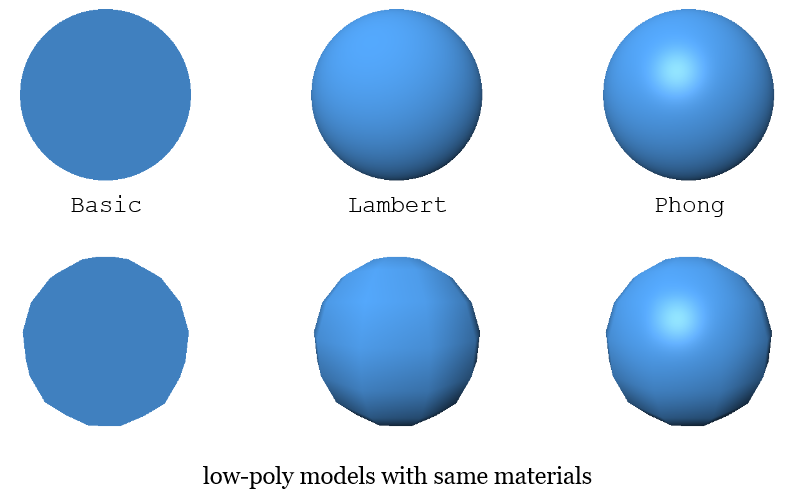
\includegraphics[width=0.9\textwidth]{images/materials.png}
    \caption{Darstellung verschiedener Materialien}
    \label{fig:my_label}
\end{figure}
\begin{itemize}
    \item Material 
    
Abstrakte Basisklasse für alle Materialien.

Definition:
\begin{lstlisting}
Material()
\end{lstlisting}
Dieser Konstruktor erstellt ein generisches Material.
\newpage

\item MeshBasicMaterial 

Ein Material um Objekte in einem primitiv texturierten Zustand darzustellen. Dies Art von Material ist nicht von Licht beeinflussbar.

Definition:
\begin{lstlisting}
MeshBasicMaterial( parameters : Object )
\end{lstlisting}
JavaScript Beispiel
\begin{lstlisting}
const myNewMaterial = new THREE.MeshBasicMaterial(
    {
        color: 'red'
    }
);
\end{lstlisting}
Ein Beispiel für die Erstellung eines MeshBasicMaterials, in dem der Parameter \textit{color} auf \textit{red} gesetzt wird. Diese Konfiguration färbt das Material rot ein. \\

\item MeshLambertMaterial 

Anders wie das MeshBasicMaterial, berechnet dieses die Reflektionen basierend auf dem \textit{Lambertsches Gesetz}. 
Das MeshLambertMaterial wird kaum dafür genutzt um realitätsgetreue Szenen darzustellen, doch durch die Einfachkeit der Reflektions- und Belichtungsmodelle ist es performanter als das MeshPongMaterial. Jedoch muss man grafische Inkorrektheiten bei der Darstellung in Kauf nehmen.

Definition:
\begin{lstlisting}
MeshLambertMaterial( parameters : Object )
\end{lstlisting}
Schatten und Reflektionen werden entlang der Achsen berechnet und visualisiert.
\newpage
\item MeshPhongMaterial 

Das MeshPhongMaterial, berechnet die Reflektionen basierend auf dem \textit{Blinn-Phong-Beleuchtungsmodell}. Schattierungen werden durch das hinzuziehen des sogenannten \textit{Phong-Shading-Models} generiert. Die Besonderheit dieser Vorgehensweise ist, dass für jeden Pixel des Objekts ein Schatten berechhnet wird, so ist das MeshPhongMaterial gut dazu geeignet realitätsgetreue Szenen darzustellen.

Definition:
\begin{lstlisting}
MeshPhongMaterial( parameters : Object )
\end{lstlisting}
\end{itemize}

\textbf{Konfiguration von Materialien:} \cite{material}

\begin{itemize}
\item Material.side \\
Die \textit{Material.side} Option lässt die Sichtbarkeit der Oberflächen konfigurieren. Der Standardwert ist \textit{THREE.FrontSide}. \\
\textbf{Arten am Beispiel eines Würfels:}\\
- THREE.FrontSide \\
Nur die Außenseiten des Würfels sind sichtbar. \\
- THREE.BackSide \\
Nur die Innenseiten des Würfels sind sichtbar. \\
- THREE.DoubleSide \\
Beide Seiten sind sichtbar. \\
\begin{figure}[h]
    \centering
    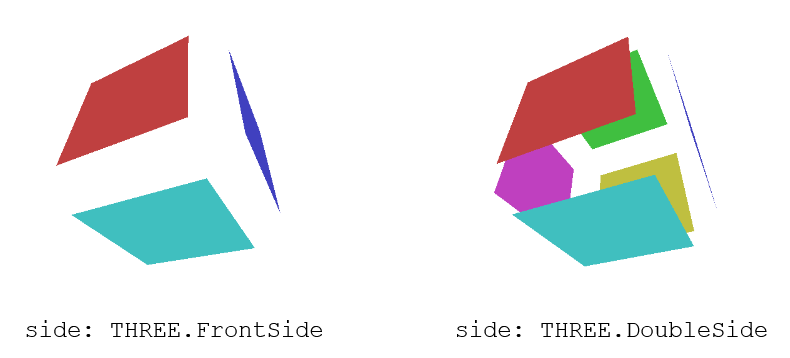
\includegraphics[width=0.9\textwidth]{images/doubleside.png}
    \caption{Material Sichtbarkeit}
    \label{fig:my_label}
\end{figure}
\newpage
\item Material.flatShading\\
Der Option \textit{Material.flatShading} wird ein boolescher Wert zugewiesen, bei \textit{true} werden die einzelnen Flächen nicht geglättet und somit sind sie sichtbar. Wenn der Wert \textit{false} ist werden die Flächen an ihren Verbindungsstellen geglättet und miteinander verbunden.\\ Der Standardwert ist \textit{false}. 
\begin{figure}[h]
    \centering
    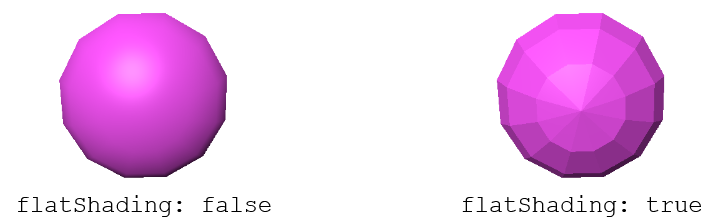
\includegraphics[width=0.9\textwidth]{images/flatShading.png}
    \caption{Material Schatten Glätte}
    \label{fig:my_label}
\end{figure}

\item Material.shininess \\
Die Option \textit{shininess} definiert den Glanz eines Materials das einem Objekt hinzugefügt wurde. Der Minimalwert ist 0 und bei dieser Konfiguration wird der Glanzeffekt deaktiviert. Der Maximalwert hingegen ist 150.\\ Der Standardwert ist \textit{30}.
\begin{figure}[h]
    \centering
    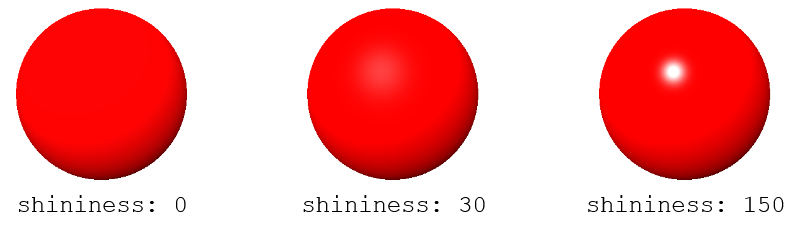
\includegraphics[width=0.8\textwidth]{images/shininess.png}
    \caption{Material Glanz}
    \label{fig:my_label}
\end{figure}
\end{itemize}
\newpage
\subsection{Objekte}
Um Geometrien und Materialien zusammenzuführen werden \textit{Objekte} oder auch \textit{Meshes} genannt, genutzt. Three.js bietet 12 unterschiedliche Arten von Objekten.\\ \\
JavaScript Initialisierung:
\begin{lstlisting}
var cube_geomtry = new THREE.BoxBufferGeometry(5, 5, 5);
var cube_material = new THREE.MeshBasicMaterial({ color: red });
var cube = new THREE.Mesh(cube_geomtry, cube_material);
scene.add(cube);
\end{lstlisting}
In diesem Beispiel-Code wird ein Objekt mit dem entsprechenden Geometrien und Materialien erstellt.\\
\begin{figure}[h]
    \centering
    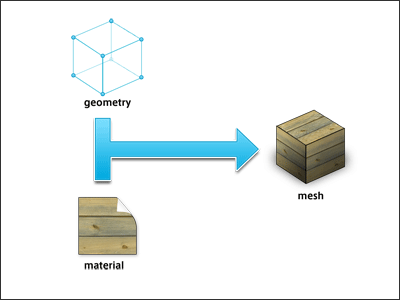
\includegraphics[width=1\textwidth]{images/geoplusmat.png}
    \caption{Geometrie + Material Illustration \cite{geoplusmat}}
    \label{fig:my_label}
\end{figure}
\newpage
\textbf{Arten:}\\
\begin{itemize}
    \item Mesh \\
Eine Klasse die es ermöglicht auf \textit{Polygonnetze} basierende Objekte zu erstellen. \\
Dem Mesh werden zwei Objekte zur Verfügung gestellt, eine Geometrie (\textit{geometry}) und ein Material (\textit{material}). \\ 
Standardwerte: BufferGeometry und MeshBasicMaterial. \\
Definition:
\begin{lstlisting}
Mesh( geometry : Geometry, material : Material )
\end{lstlisting}
    \item Line \\
Dieser Objekttyp visualisiert Linien, die im Vektorformat festgelegt werden. \\
Definition:
\begin{lstlisting}
LineSegments( geometry : Geometry, material : Material )
\end{lstlisting}
JavaScript Beispiel:
\begin{lstlisting}
var material = new THREE.LineBasicMaterial(
                    {color: white}
                );

var geometry = new THREE.Geometry();
geometry.vertices.push(
	new THREE.Vector3( -10, 0, 0 ),
	new THREE.Vector3( 0, 10, 0 ),
	new THREE.Vector3( 10, 0, 0 )
);

var line = new THREE.Line( geometry, material );
scene.add( line );
\end{lstlisting}
    \item Points \\ 
Mit der Klasse \textit{Points} kann man Punkte visualisieren.

Definition:
\begin{lstlisting}
Points( geometry : Geometry, material : Material )
\end{lstlisting}
\end{itemize}
\newpage
\subsection{Textur}
Um Materialien mit einer komplexeren Struktur zu nutzen werden Texturen genutzt. \\
Texturen werden Three.js mit .PNG oder .JPG - Dateien bereitgestellt.

\begin{itemize}
    \item TextureLoader 
  
 Der TextureLoader bietet die Möglichkeit bereitgestellte Bilddateien in eine sogenannte Material - \textit{Map} einzubetten. Die folgenden Code - Beispiele zeigen die Handhabung des TextureLoaders mit einem Bild im .JPG Format. \cite{TextureLoader}
 
Definition:
\begin{lstlisting}
TextureLoader( manager : LoadingManager )
\end{lstlisting}

Laden einer Textur: 
\begin{lstlisting}
var texture = new THREE.TextureLoader().load( 'textures/wand.jpg' );
\end{lstlisting}
Mit der \textit{load} - Funktion des \textit{TextureLoaders} können beliebige Bilder in eine Variable geladen und abgespeichert werden.

Geladene Textur in Material einbetten:
\begin{lstlisting}
var wand_material = new THREE.MeshBasicMaterial( { map: texture } );
\end{lstlisting}

Dem dazugehörigen Objekt das Material zuweisen:
\begin{lstlisting}
var wand_geometrie = new THREE.BoxBufferGeometry(5, 273, 727);
var wand = new THREE.Mesh(geometry_wall, wand_material);
\end{lstlisting}

\begin{figure}[h]
    \centering
    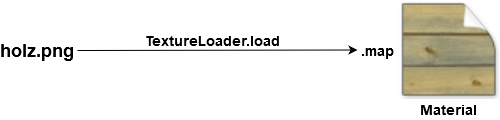
\includegraphics[width=0.9\textwidth]{images/textures.png}
    \caption{Illustration zum Texturen laden}
    \label{fig:my_label}
\end{figure}
\newpage
\item .load

In diesem Beispiel der \textit{load} - Funktion des TextureLoaders wird mit Callbacks auf den Abschluss des Ladevorgangs gewartet. Außerdem kann mit Callbacks auf Fehler reagiert werden. 

\begin{itemize}
    \item Definition 

\begin{lstlisting}
.load ( url : String, onLoad : Function,
        onProgress : Function,
        onError : Function ) : Texture
\end{lstlisting}

Die Funktionen onLoad, onProgress und onError werden dann aufgerufen wenn jeweils die Textur fertig geladen wurde, der Ladevorgang weiter fortgeschritten ist oder fehlgeschlagen hat. \\
Der Rückgabewert der \textit{load} - Funktion ist ein \textit{Texture} - Objekt.

\item JavaScript - Beispiel
\begin{lstlisting}
 // load a resource
 loader.load(
    // resource URL
    'textures/wand.jpg',

    // onLoad callback
    function ( texture ) {
        // create material
        var material = new THREE.MeshBasicMaterial( {
            map: texture
        } );
    },

    // onProgress callback currently not supported
    undefined,

    // onError callback
    function ( err ) {
        console.error( 'An error happened.' );
    }
 );
\end{lstlisting}
\end{itemize}
\end{itemize}

\newpage
\clearpage
\subsection{Kamera}
Die Kamera wird dem Renderer mitgegeben und außerdem der Szene hinzugefügt.
\\
Definition:
\begin{lstlisting}
PerspectiveCamera( fov : Number, aspect : Number,
near : Number, far : Number )
\end{lstlisting}
\begin{figure}[h]
    \centering
    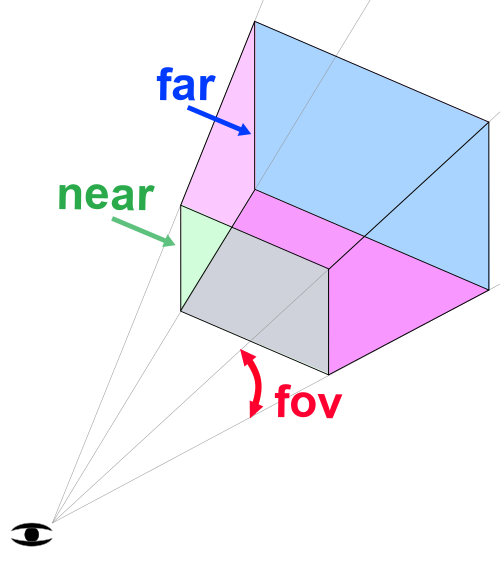
\includegraphics[width=0.6\textwidth]{images/threejs-camera.png}
    \caption{Kamera Blickwinkel \cite{fundamentals_camera}}
    \label{fig:my_label}
\end{figure}
Der Parameter \textit{fov} steht für \textit{field of view} und gibt den Winkel der Kameraaufnahmen an, vergleichbar mit unterschiedlichen Objektiven bei Kameras in der Realität.
\textit{aspect} definiert das Seitenverhältnis der Darstellung. 
\textit{near} und \textit{far} repräsentiert den Bereich vor der Kamera, der gerendert wird. Alle Objekte die nicht in diesem Bereich liegen werden abgeschnitten, oder nicht dargestellt. 
\\
JavaScript Initialisierung:
\begin{lstlisting}
camera = new THREE.PerspectiveCamera(50, 
window.innerWidth / window.innerHeight, 1, 10000);
scene.add(camera);
\end{lstlisting}
\newpage 
\textbf{Arten:}  \cite{Camera_Types}
\begin{itemize}
    \item ArrayCamera 
  
Eine Instanz der ArrayCamera beinhaltet ein Array von Kamera-Instanzen, sie wird genutzt um Szenen effizienter zu rendern. Dieses Element wird hauptsächlich für die Visualisierung von Virtual Reality Szenen genutzt.

Definition:
\begin{lstlisting}
ArrayCamera( array : Array )
\end{lstlisting}
    \item CubeCamera 
  
Dieser Konstruktor erstellt und beinhaltet sechs PerspectiveCameras, die dann ein WebGLCubeRenderTarget \cite{WebGLCubeRenderTarget} rendern und darstellen können.

Definition:
\begin{lstlisting}
CubeCamera( near : Number, far : Number,
cubeResolution : Number, options : Object )
\end{lstlisting}
    \item PerspectiveCamera 
  
Die PerspectiveCamera bietet dem Nutzer eine Ansicht die der Realität am nähesten kommt. Perspektiven können mit diesem Element am besten abgebildet werden. Der Blickwinkel wird in einer Kegelform generiert. Diese Kamera wird im Bad-Designer genutzt, da die Illusion erschaffen werden soll, direkt vom Bad zu stehen. \cite{Camera_Types}
Definition:
\begin{lstlisting}
PerspectiveCamera( fov : Number, aspect : Number,
near : Number, far : Number )
\end{lstlisting}
\newpage
\begin{figure}[h]
    \centering
    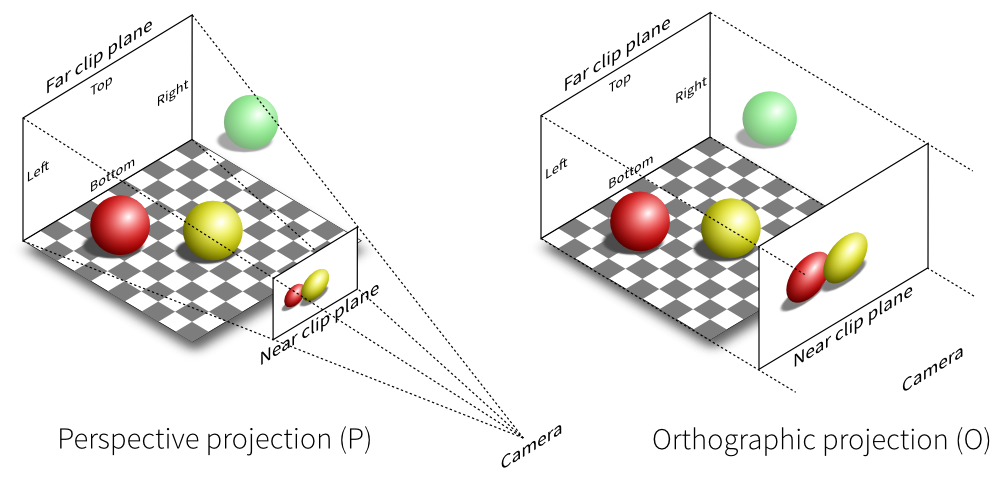
\includegraphics[width=0.9\textwidth]{images/orthographicVsPerspective.png}
    \caption{PerspectiveCamera und OrthographicCamera \cite{orthographicVsPerspective}}
    \label{fig:my_label}
\end{figure}
\item OrthographicCamera 
  
Im Gegensatz zur PerspectiveCamera generiert die OrthographicCamera keinen kegelförmigen sondern einen quaderförmigen Blickwinkel, durch diese Darstellung ist es nicht möglich Perspektiven zu gestalten. Die dargestellten Bilder der Kamera sind vergleichbar mit dem betrachten eines Bildes mit einer Lupe.

Definition:
\begin{lstlisting}
OrthographicCamera( left : Number, right : Number, 
top : Number, bottom : Number, 
near : Number, far : Number )
\end{lstlisting}
\end{itemize}
\subsection{Steuerung}
Eine Kamera macht es dem Benutzer nur möglich die Szene zu begutachten, wenn die Kamera bewegt werde will muss eine Steuerung definiert werden. \\ Three.js bietet acht verschiedene Steuerungselemente. \\
\textbf{Verwendung} \\
Im Bad-Designer wird ein Steuerungselement namens \textit{OrbitControls} genutzt, um bei der 
frontalen Ansicht der Module, die Kamera, vergleichbar zum Kopf des Menschen, schwenkbar zu machen. \\
Außerdem ist dieses Steuerungselement maßgeblich dafür verantwortlich das in Animationen in der die Kamera bewegt wird [\ref{sec:Kamera - Animationen}], ein Fokus gesetzt werden kann.
\newpage
\textbf{Arten:}  \cite{OrbitControls}
\begin{itemize}
    \item OrbitControls 
  
Die OrbitControls ermöglichen es die Kamera in einer Kreisbahn um einen bestimmten Punkt zu bewegen. 

Definition:
\begin{lstlisting}
OrbitControls( object : Camera, domElement : HTMLDOMElement )
\end{lstlisting}
Der Parameter \textit{object} ist unbedingt erforderlich und diesem muss eine Instanz der Klasse \textit{Camera} zugewiesen werden. So weiß das Steuerungs - Objekt welche Kameraeinstellungen verändert werden müssen und welche Kamera kontrolliert wird. \\
Dem zweite Parameter, \textit{domElement}, kann ein \textit{HTMLDOMElement} zugewiesen werden. Dies ermöglicht es Eventlistener zu definieren. 
\item DeviceOrientationControls

Die DeviceOrientationControls werden dafür genutzt um die Kamera, basierend auf die Ausrichtung eines mobilen Gerätes, zu steuern.

Definition:
\begin{lstlisting}
DeviceOrientationControls( object : Camera )
\end{lstlisting}
\item FlyControls

Die FlyControls ermöglichen es den Nutzer die Kamera wie ein Flugzeug zu steuern. Durch Bewegung der Maus wird die Kamera nach links oder rechts geschwenkt und außerdem wird die Kamera so nach vorne bewegt, dass der Effekt entsteht das diese im Raum herumfliegt.

Definition:
\begin{lstlisting}
FlyControls( object : Camera, domElement : HTMLDOMElement )
\end{lstlisting}
\end{itemize}
\newpage
\subsection{Licht}
Um Objekte und Elemente für die Kamera sichtbar zu machen muss der Szene eine Lichtquelle hinzugefügt werden. Three.js bietet zahlreiche Arten von Lichtern, die viele Möglichkeiten bieten um die verschiedensten Effekte einzubauen.
\\
\\
\textbf{Arten:} \cite{how_3d_works}
\begin{figure}[h]
    \centering
    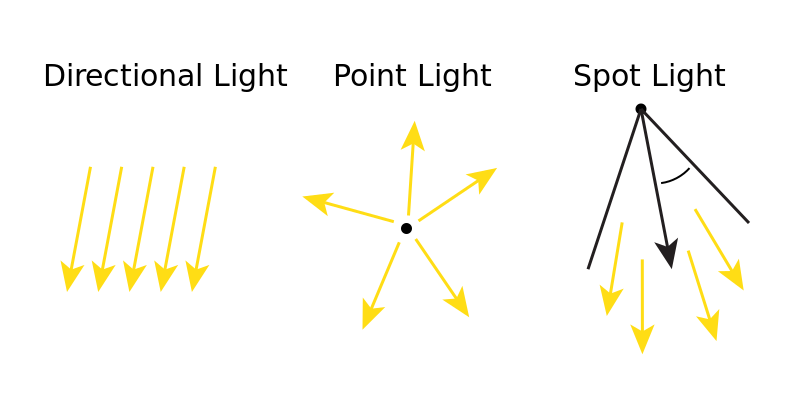
\includegraphics[width=1\textwidth]{images/lights.png}
    \caption{Directional-, Point- und Spot-Light \cite{types_of_lights_image}}
    \label{fig:my_label}
\end{figure}
\begin{itemize}
  \item DirectionalLight
  
Das DirectionalLight kann mit Sonnenlicht verglichen werden, es kann an keine konkrete Position gesetzt werden und ist mit einer Lichtquelle die sich in sehr großer Entfernung liegt gleichzusetzen.

Definition:
\begin{lstlisting}
DirectionalLight( color : Integer, intensity : Float )
\end{lstlisting}
  \item AmbientLight 
  
Dem AmbientLight auch Umgebungslicht genannt, kann keine Position zugewiesen werden und es erhellt alle Objekte gleichmäßig.

Definition:
\begin{lstlisting}
AmbientLight( color : Integer, intensity : Float )
\end{lstlisting}
\newpage
\item PointLight
  
Das Pointlight kann mit einer Glühbirne verglichen werden, da das Licht in alle Richtungen abgestrahlt wird, außerdem kann eine Position festgelegt werden.

Definition:
\begin{lstlisting}
PointLight( color : Integer, intensity : Float, 
distance : Number, decay : Float )
\end{lstlisting}
\item SpotLight

Das SpotLight kann mit einer Taschenlampe verglichen werden, da das Licht in einem Kegel vom definierten Bereich ausgestrahlt wird. 

Definition:
\begin{lstlisting}
SpotLight( color : Integer, 
intensity : Float, distance : Float, 
angle : Radians, penumbra : Float, decay : Float )
\end{lstlisting}
  \item HemisphereLight
  
Das HemisphereLight imitiert realistisches Sonnenlicht, durch Definierung der Himmels- und Bodenfarben werden Verfärbungen und Reflektionen auf den Objekten generiert.

Definition:
\begin{lstlisting}
HemisphereLight( skyColor : Integer, 
groundColor : Integer, intensity : Float )
\end{lstlisting}
  \item RectAreaLight
  
Das RectAreaLight emittiert Licht entlang einer rechteckigen Linie, es kann dafür benutzt werden um helle Fenster oder LED-Streifen zu visualisieren.

Definition:
\begin{lstlisting}
RectAreaLight( color : Integer, intensity : Float, 
width : Float, height : Float )
\end{lstlisting}
\end{itemize}
\clearpage \newpage
\subsection{Loader}\label{sec:Loader}
\textbf{Arten:} \\
\begin{itemize}
    \item Loader \cite{three.js_loader}\\
    Die Klasse Loader ist die Basisklasse von der die darunter folgenden Loader-Klassen erben.
    
    Konstruktor:
    \begin{lstlisting}
Loader( manager : LoadingManager )
    \end{lstlisting}
    
    
    \item ObjectLoader \cite{three.js_objectLoader}\\
    Der ObjectLoader lädt eine JSON-Resource in ein JSON Objekt beziehungsweise in eine Szene. Dieser Loader verwendet intern einen FileLoader um eine JSON-Datei einzulesen, danach kann es einem Objekt gespeichet werden.
    
    Konstruktor:
    \begin{lstlisting}
ObjectLoader( manager : LoadingManager )
    \end{lstlisting}
    
    
    \item TextureLoader \cite{three.js_TextureLoader}\\
    Diese Klasse dient um eine Texture auf ein Objekt zu laden. Intern verwendet sie einen ImageLoader der .jpg oder .png Dateien lädt und sie anschließend auf das Objekt anwendet.
    
    Konstruktor:
    \begin{lstlisting}
TextureLoader( manager : LoadingManager )
    \end{lstlisting}
    
    
    \item MaterialLoader \cite{three.js_materialLoader}\\
    Der MaterialLoader ermöglicht es Materials im JSON-Format zu laden. Materials sind beschreiben das Aussehen eines Objektes. Der Loader verwendet intern einen FileLoader für das Laden der Materials die beispielsweise in einer JSON-Datei vorliegen. 
    
    Konstruktor:
    \begin{lstlisting}
MaterialLoader( manager : LoadingManager )
    \end{lstlisting}
    
    
    \item AnimationLoader \cite{three.js_AnimationLoader}\\
    Für das Laden von AnimationClips im JSON-Format wird der AnimationLoader verwendet. Ein AnimationClip ist wiederverwendbarer Satz von einer Animationsreihenfolge. Auch der AnimationLoader setzt intern auf einen FileLoader der gegebenenfalls eine JavaScript-Datei [\ref{sec:JavaScript}] mit Animationen lädt. 
    
    Konstruktor:
    \begin{lstlisting}
AnimationLoader( manager : LoadingManager )
    \end{lstlisting}
    
    \item GLTFLoader \cite{three.js_GLTFLoader}\\
    Die Abkürzung glTF steht für Graphics Library Transmission Format. Wie der Name schon vermuten lässt ist es eine offene Format-Spezifikation für effiziente Übertragung und Laden von dreidimensionalen Objekten.
    
    Konstruktor:
    \begin{lstlisting}
GLTFLoader( manager : LoadingManager )
    \end{lstlisting}
    
    \item DRACOLoader \label{dracoloader} \cite{three.js_DRACOLoader}\\
    Draco ist eine quelloffene Bibliothek für das Komprimieren und Dekomprimieren von 3D Objekten. Komprimierte Objekte können dadurch erheblich weniger Speicher benötigen aber zu lasten der Dekomprimierung am Client. Typischerweise besitzen Draco-Dateien Eckpunkte, Normalen, Farben und andere Attribute jedoch keine Materials, Texturen oder Animationen. Um davon Gebrauch zu machen kann man sie in eine glTF-Datei umwandeln. Werden Draco und glTF kombiniert wird ein DRACOLoader intern von einem GLTFLoader verwendet. 

    Konstruktor:
    \begin{lstlisting}
DRACOLoader( manager : LoadingManager )
    \end{lstlisting}
    
    \item OBJLoader \cite{three.js_OBJLoader}\\
    Diese Klasse liest .obj Dateien ein. Diese simplen Dateien beinhalten dreidimensionale Geometrie in einem für Menschen lesbaren Format. Dabei werden die Koordinaten, Eckpunkte und Texturen abgespeichert. 
    
    Konstruktor:
    \begin{lstlisting}
OBJLoader( manager : LoadingManager )
    \end{lstlisting}
    
    \item MTLLoader \cite{three.js_MTLLoader}\\
    Dieser Loader dient ausschließlich für das Laden von .mtl Resourcen. Das Material Template Library Format ist eine Hilfsdatei für eine .obj Datei, die Attribute wie den Schatten oder Materials zu einem Objekt. Der MTLLoader wird intern vom OBJLoader verwendet.
    
    Konstruktor:
    \begin{lstlisting}
MTLLoader( loadingManager : LoadingManager )
    \end{lstlisting}
\end{itemize}
\clearpage \newpage
\subsection{LoadingManager}
Der LoadingManager verarbeitet und verfolgt geladene und ausstehende Daten. \\ Wenn ein Loader instanziiert wird, verwendet dieser eine globale Standardinstanz: \textit{DefaultLoadingManager}. \cite{LoadingManager} \\ \\
Definition:
\begin{lstlisting}
LoadingManager( onLoad : Function,
                onProgress : Function,
                onError : Function )
\end{lstlisting}
\begin{itemize}
    \item onStart: Wird aufgerufen wenn der Ladevorgang beginnt. 
    \item onLoad: Wird aufgerufen wenn alle Loader den Ladevorgang abgeschlossen haben. 
    \item onProgress: Wird aufgerufen wenn ein einzelnes Element fertig geladen wurde. 
    \item onError: Wird aufgerufen wenn ein Loader einen Fehler verursacht.
\end{itemize}
JavaScript - Beispiel:
\begin{lstlisting}
var manager = new THREE.LoadingManager();
manager.onStart = function ( url, itemsLoaded, itemsTotal ) {
    console.log( 'Started loading file: ' + url);
};

manager.onLoad = function ( ) {
    console.log( 'Loading complete!');
};

manager.onProgress = function ( url, itemsLoaded, itemsTotal ) {
    console.log( 'Loading file: ' + url);

};
\end{lstlisting}
Dem LoadingManager einem Loader zuweisen:
\begin{lstlisting}
var loader = new THREE.OBJLoader( manager );
loader.load( 'file.obj');
\end{lstlisting}

\newpage
\clearpage
\section{tween.js}\label{sec:tween.js}
\cite{tween.js_tutorial}\cite{tween.js_GitHub}\cite{tween.js_createjs}
\section*{Erläuterung}
tween.js ist eine auf JavaScript [\ref{sec:JavaScript}] basierende Bibliothek die für Animation und Tweening verwendet wird. Unter Tweening versteht man das Verfahren zur Erzeugung von Einzelbildern zwischen Schlüsselbildern um einen flüssigen Ablauf zu suggerieren. Außerdem ist tween.js ein Standard für Animationen im Zusammenspiel mit three.js [\ref{sec:three.js}]. Für die nötige Schnelligkeit, einfache Handhabung und Flüssigkeit ist im Hintergrund das chaining zuständig. Das chainen also anketten ermöglicht es Animationen hintereinander ablaufen zu lassen und Endlosschleifen zu erstellen. 

\section*{Funktionalität}
Das Einbinden der Bibliothek erfolgt JavaScript typisch über einen Link oder Installation per npm.
Das tween.js Projekt wird auf GitHub [\ref{sec:Git}] gehostet und unter der MIT-Lizenz [\ref{sec:MIT}] zur Verfügung gestellt.

\section*{Verwendung}
Das Einfliegen der Badezimmerelemente und animieren der Detailansichten werden allesamt von tween.js abgewickelt. Dabei müssen nur ein Tween Objekt erstellt werden und das zu animierende Element übergebene werden. Anschließend kann man eine vordefinierte Animation auswählen und bestimmen von wo beziehungsweise wohin etwas animiert werden soll und in welcher Zeitspanne. Ein Code Beispiel folgt auf der nächsten Seite.

\newpage \clearpage
\section*{Code Beispiel zu tween.js}
\begin{lstlisting}
// Erstellen eines Tween Objektes
    var position = { x : 0, y: 300 };
    var target = { x : 400, y: 50 };
    var timeToAnimate = 2000; //in ms
    var tween = new TWEEN.Tween(position).to(target, timeToAnimate);
    
// Was soll beim animieren passieren?    
    tween.onUpdate(function(){
    mesh.position.x = position.x;
    mesh.position.y = position.y;
    });
    
// Animationstyp setzen    
    tween.easing(TWEEN.Easing.Elastic.InOut)

// Animation starten
    tween.start();

// Endlosschleife erstellen
    tweenHead.chain(tweenBack);
    tweenBack.chain(tweenHead);
\end{lstlisting}

\newpage
\clearpage

\section{jQuery}
\cite{jQuery}
\section*{Erläuterung}
JQuery ist die meistverwendete und freie JavaScript-Bibliothek die für Manipulationen und Navigation per DOM (Document Object Model) entwickelt wurde. Die plattformunabhängige Bibliothek ist das erste Mal 2006 unter der MIT-Lizenz [\ref{sec:MIT}] erschienen. 74\% der 10.000 meistbesuchten Websites ~\cite{jQuery_Usage01} und bereits jede zweite Seite ~\cite{jQuery_Usage02}  nutzen jQuery. Des Weiteren werden Webframeworks und Content-Management-Systeme wie WordPress, Joomla und Drupal mit jQuery ausgeliefert, die zusätzlich zur Beliebtheit beitragen. 

\section*{Funktionalität}
JQuery ist eine schnelle, leichtgewichtige und funktionsreiche JavaScript-Bibliothek die Dinge wie das Event Handling, Animationen und AJAX vereinfacht. Multiple Browser unterstützen diese Bibliothek und ist somit plattformunabhängig.

\section*{Verwendung}
JQuery wird primär im Bad-Designer für das Wählen von HTML-Elementen im JS-Code [\ref{sec:JavaScript}] angewendet. Dadurch kann man auf die Attribute und das Styling von Objekten via jQuery zugreifen und diese dynamisch manipulieren. 

\newpage
\clearpage

\section{Bootstrap}
\cite{BootStrap_Website} \cite{BootStrap_About}
\section*{Erläuterung}
Bootstrap ist ein quelloffenes Frontend-CSS-Framework. Die Technologie bietet verschiedenste Designvorlagen für gängige HTML-Elemente wie Buttons, Tabellen, Typografie, Formulare, et cetera  und optional auch JavaScript-Erweiterungen [\ref{sec:JavaScript}]. Der Entwickler von Bootstrap ist der Kurznachrichtendienst Twitter. Das Toolkit ist das erste Mal 2011 unter der MIT-Lizenz [\ref{sec:MIT}] erschienen. Jedoch ist nur der in HTML, CSS und JavaScript geschriebene Code unter der MIT-Lizenz erhältlich. Bootstrap wird als quelloffenes Framework auf GitHub [\ref{sec:Git}] gehostet.Laut eigenen Angaben des Unternehmens ist Bootstrap die beliebteste HTML, CSS und JavaScript Bibliothek der Welt.

\section*{Funktionalität}
Das Framework ist grundsätzlich modular aufgebaut und besteht im wesentlichen aus Stylesheets, die die einzelnen Komponenten beinhalten. Diese wiederum werden in einer zentralen Bootstrap-Datei kumuliert. Dieser Architektur ist es zu verdanken dass Entwickler durch Manipulationen der Bootstrap-Datei entscheiden welche Komponenten verwendet werden. Einzelne Attribute wie zum Beispiel die Schriftart und Größe können in einem gebündeltem Konfigurationsstylesheet geändert werden. Ab der Version 2.0 kann der Entwickler über ein Formular gewünschte Komponenten anpassen und anschließend wird eine fertig kompilierte CSS-Datei generiert. 
\section*{Verwendung}
Das Design der Website des Bad-Designers wurde mit Bootstrap realisiert und einige JavaScript Funktionen.

\newpage
\clearpage 

\section{NGINX}\label{sec:NGINX}
\cite{nginx_wiki} \cite{wiki_nginx}
\section*{Erläuterung} 
NGINX ist eine modular aufgebaute Webserver-Software, die von Igor Sysoev entwickelt wurde. Sie wird unter der BSD-Lizenz[\ref{sec:BSD}] entwickelt. Die Software ist das erste Mal Ende 2004 erschienen und wird bis heute in regelmäßigen Abständen aktualisiert und weiterentwickelt. Außerdem wurde er in der weitverbreiteten und robusten Programmiersprache C geschrieben.

\section*{Funktionalität}
Der Webserver bietet durch den modularen Aufbau eine Vielzahl an möglichen Techniken, wie zum Beispiel Lastverteilung, Reverse proxying, SSL, Flash-Video-Streaming, WebSocket-Protokoll und vieles mehr. 

\section*{Verwendung}
NGINX gehört zu den marktführen und wird heutzutage bei rund
 42\% der 1.000 Webseiten ~\cite{nginxWorldWide} mit dem höchsten Traffic verwendet. 
 Als http-Server hat er in Österreich sogar knapp 10\% Marktanteil ~\cite{nginxAT}. 
\\
Der Webserver dient beim Bad-Designer als Back-End wo die ganzen Modelle vom Bad und die Website selbst gehostet werden.




\clearpage
\newpage

\section{AutoCAD}
\small{\cite{wiki_autocad}}
\section*{Erläuterung}
AutoCAD ist ein von AutoDesk entwickelter grafischer Zeichungseditor. Dieser ermöglicht es speziell technische Zeichnungen zu modellieren. Außerdem ist es ein vektororientiertes Zeichentool, das auf den Grundlagen für komplizierte 3D-Objekte basiert wie Linien, Polylinien, Kreisen, Bögen und Texten.
\\
Durch die umfangreichen 3D-Funktionen findet das Programm primär in den Bereichen Maschinenbau, Architektur, Design, Geoinformatik häufig Verwendung. In den genannten Bereichen ist die Software konstitutiv und manche Bauwerke beziehungsweise Maschinen sind erst dadurch möglich gewesen.

\section*{Funktionalität}
Die von der Firma AutoDesk entwickelten Dateiformate .dwg sowie .dxf sind mittlerweile ein Industriestandard im Austausch von CAD-Daten. Dies ermöglicht es das die Dateien auf den verschiedensten Plattformen wie Windows, Unix und MacOS mit Hilfe des Editors verwendbar sind. Desweitern kann man es auch als WebApp und Mobile App für Smartphones und Tablets verwenden.

\section*{Verwendung}
Alle Module des Badezimmers sind in AutoCAD modelliert worden. Von den Registern bis hin zu den Modulen des Bades. Die sanitären Anlagen wurden von der Firma {\projectpartner} zur Verfügung gestellt.

\begin{figure}[!b]
	\begin{center}
		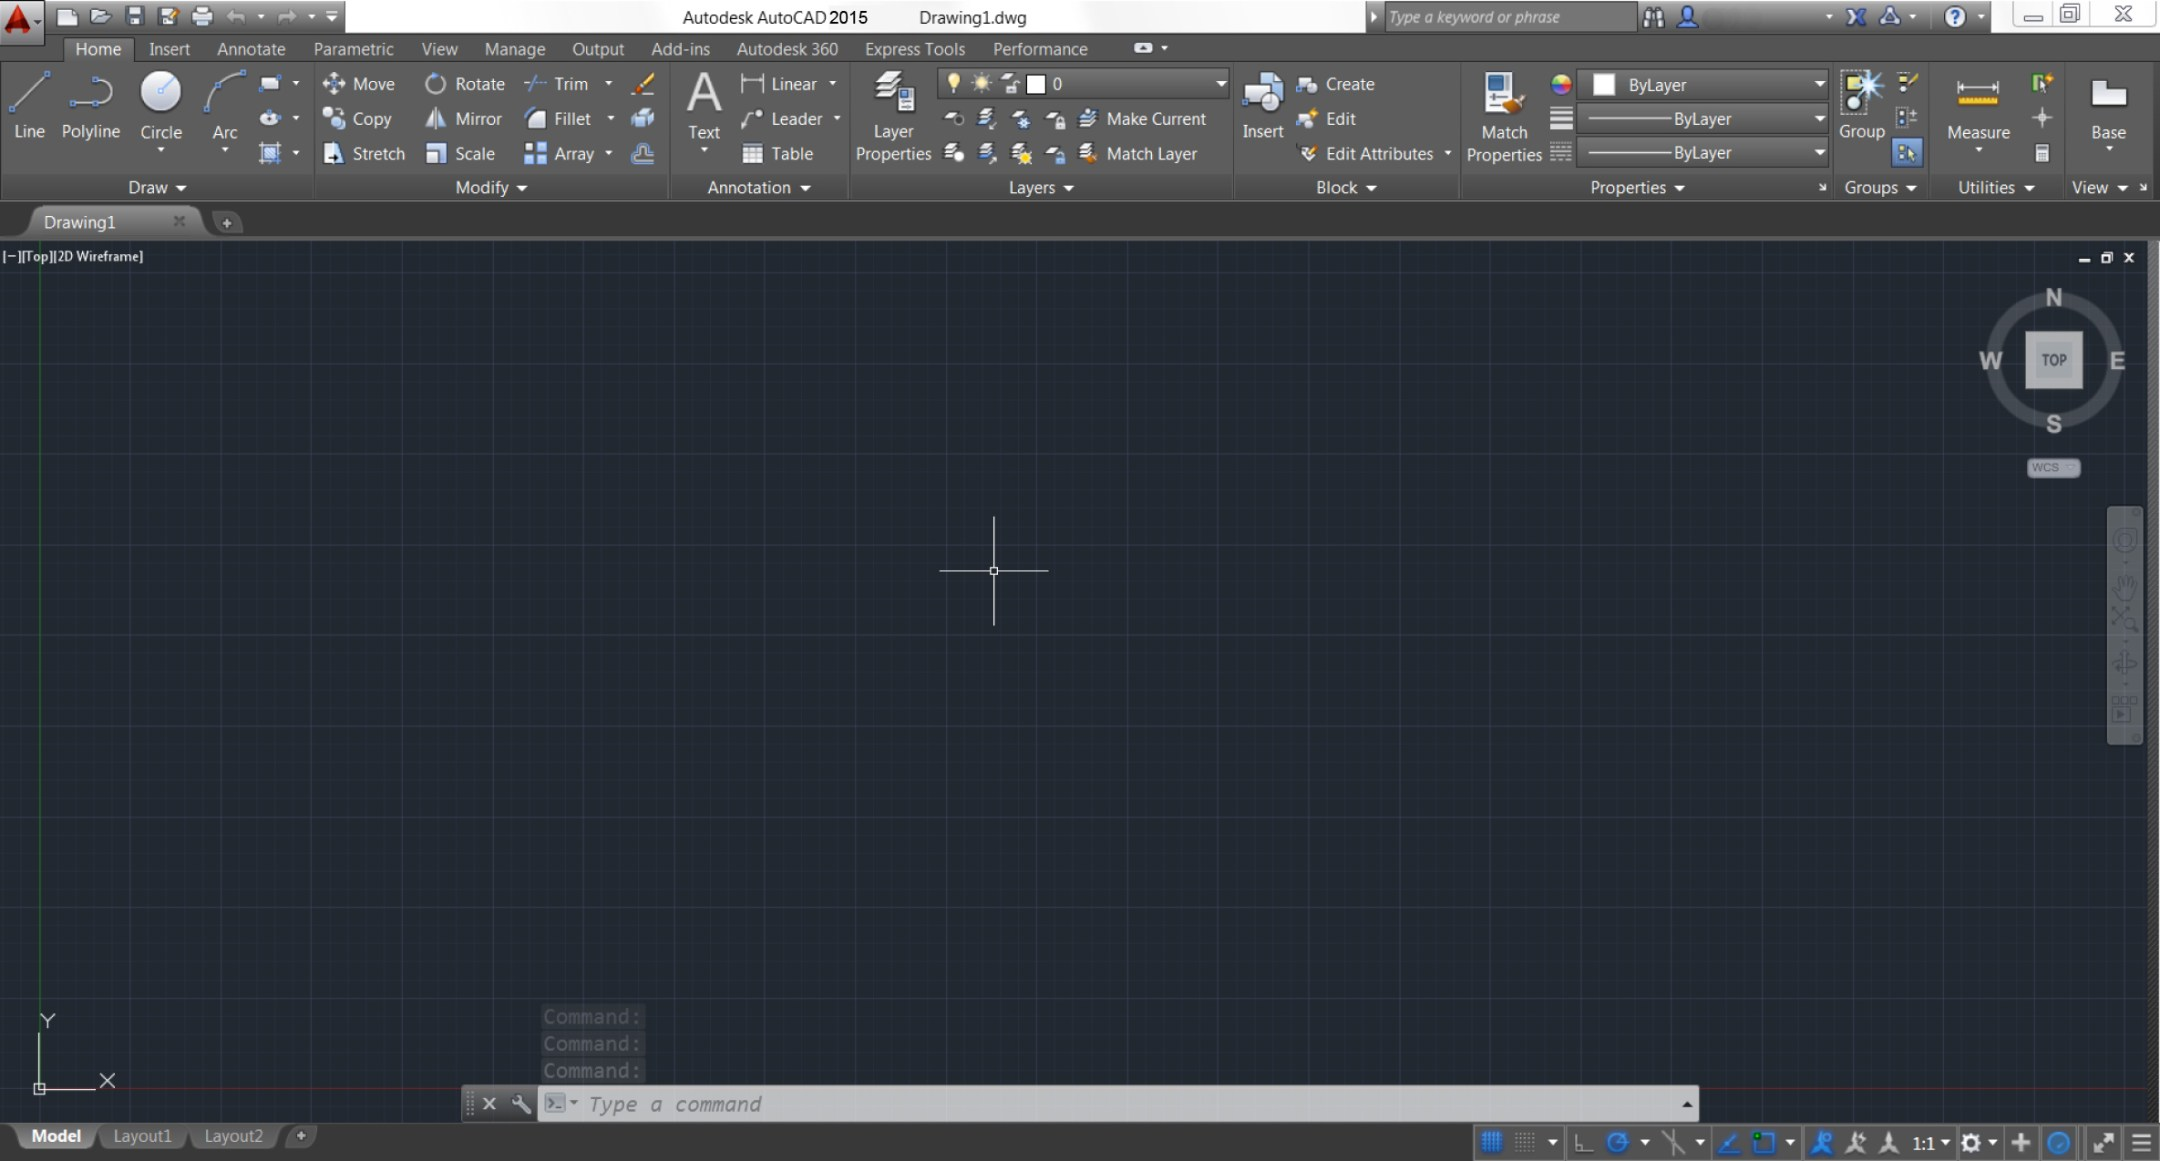
\includegraphics[width=0.7\linewidth]{images/AutoCAD_UI.jpg}
		\caption{AutoCAD UI ~\cite{autocad}}
	\end{center}
\end{figure}


\newpage
\clearpage

\section{Electron}\label{sec:Electron}
\cite{electron_doc}
\section*{Erläuterung}
Electron ist ein auf C++ und JavaScript basierendes quelloffenes Framework entwickelt von GitHub. Das 2013 erstmals erschienene Framework wird unter der MIT-Lizenz [\ref{sec:MIT}] vertrieben. Die auf Chromium und Node.js basierende Architektur ermöglicht es eine Cross-Platform-Desktop-Anwendung zu realisieren.

\section*{Funktionalität}
Webseiten die in HTML, CSS und JavaScript geschrieben wurden, können mit Electron in Desktop Anwendung umgewandelt werden ohne erheblichen Aufwand. Des Weiteren ist es möglich mit anderen Frameworks wie Vue.js und Angular zu arbeiten und anschließend zu einer Desktop App konvertieren. Das besondere daran ist, dass alle Electron-Executable auf den Betriebssystemen Windows, MacOS und Linux einwandfrei ohne Zutun ausführbar sind.


\section*{Verwendung}
Viele weitverbreitete und bekannte Programme wie die beliebten Editoren Atom und VS Code wurden mit Electron erstellt. Das Framework erlaubt es den Bad-Designer ohne eine Internetverbindung und lokal auf dem Rechner laufen zu lassen. Dafür muss nur das Executable heruntergeladen werden und schon ist es einsatzbereit. Der BadDesigner kann sowohl auf Windows als auch auf MacOS installiert und ausgeführt werden.
\begin{figure}[!b]
	\begin{center}
		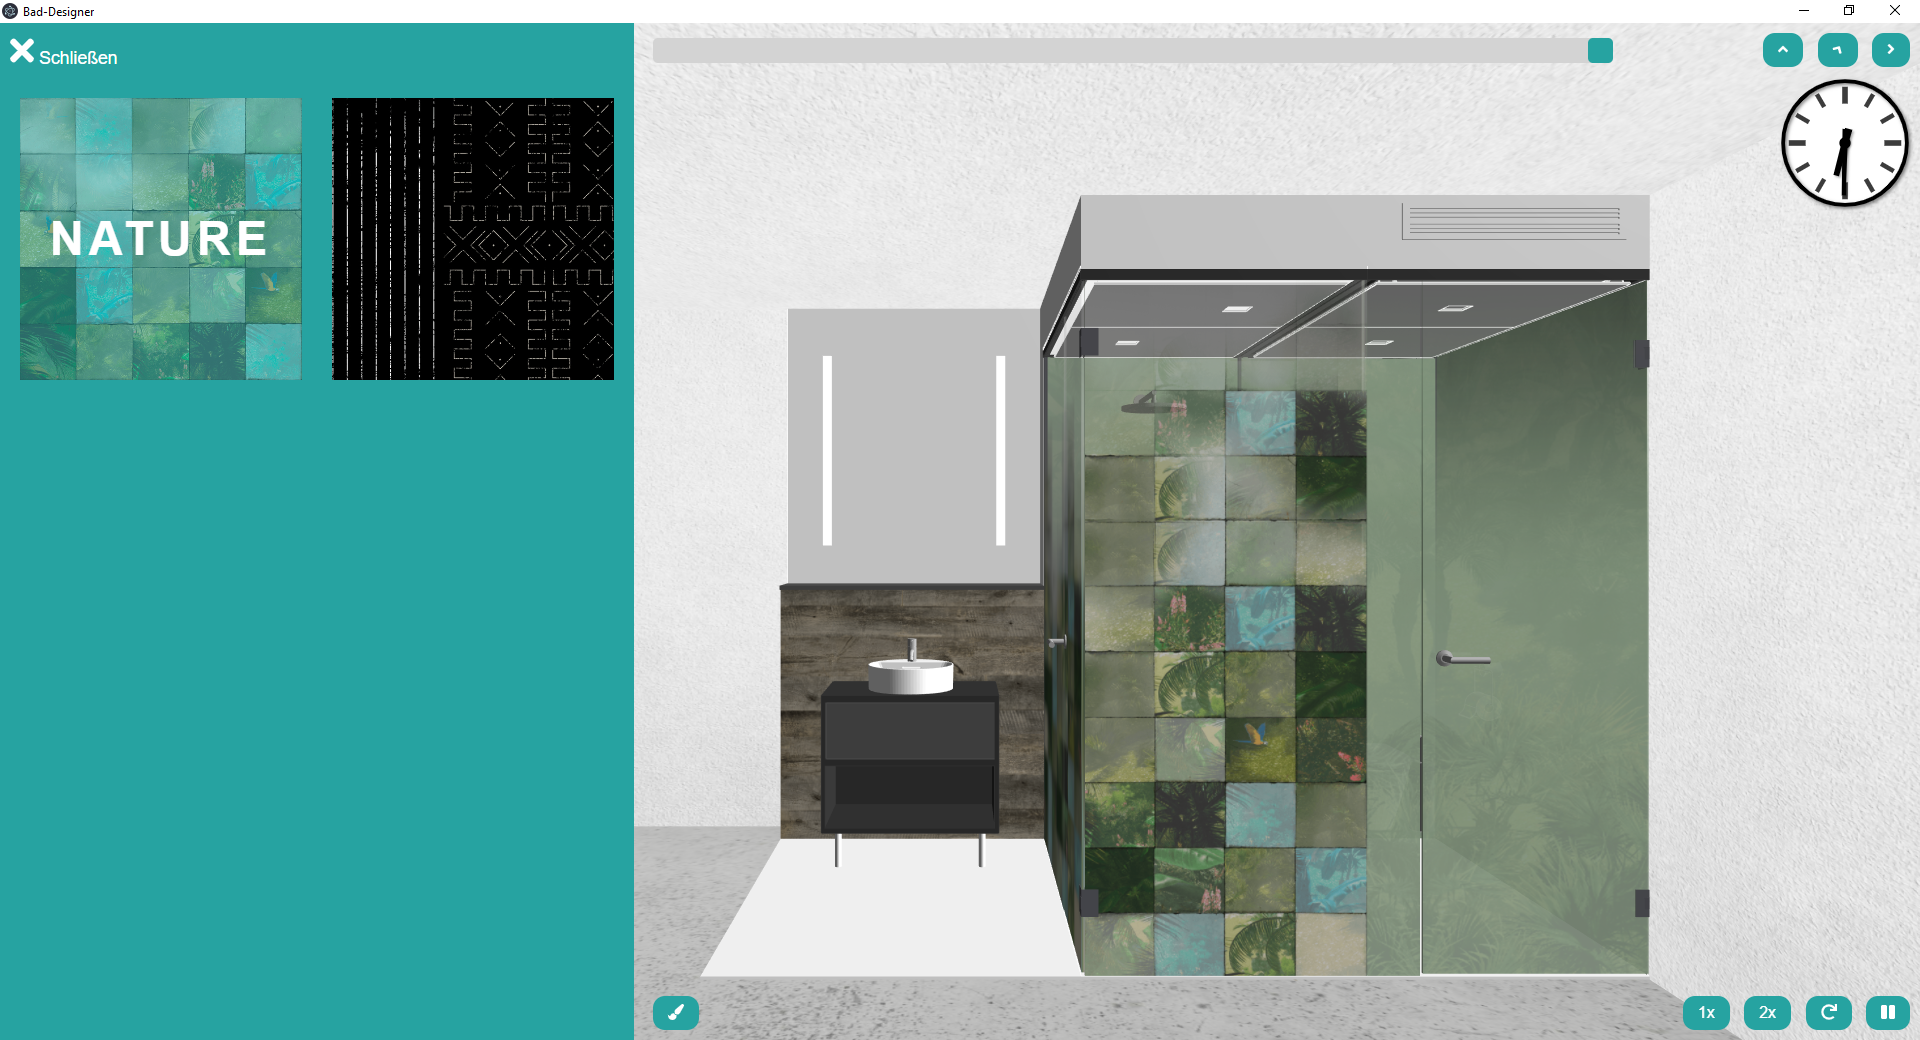
\includegraphics[width=0.9\linewidth]{images/Electron_BD.png}
		\caption{Bad-Designer als Electron Anwendung}
	\end{center}
\end{figure}


\newpage
\clearpage
\section{Git}\label{sec:Git}
\small{\cite{git_about}}
\section*{Historie}
Git ist eine kostenlose Software, die für die verteilte Versionsverteilung von Dateien entwickelt wurde. Git wurde vom Linux-Kernel-Entwickler Linus Torvalds initiiert und entwickelt. Torvalds kam auf diese Idee da er zuvor BitKeeper nutzte, diese aber durch Lizenzänderungen kostenpflichtig wurde. 2005 begann er mit der Entwicklung des beliebten Versionsverwaltungsprogrammes. Dabei hatte er drei Anforderungen. Er wollte Unterstützung verteilter Arbeitsläufe, hohe Sicherheit gegen Verfälschung und hohe Effizienz. Mittlerweile ist der Maintainer Junio Hamano. 2018 wurde GitHub für 7,5 Milliarden US-Dollar von Microsoft übernommen. \\
Git läuft auf den Betriebssystemen Linux, MacOS und Windows. Das Programm selbst wurde in den Sprachen C, Perl, Tcl, Python und C++ geschrieben und unter der GNU-Lizenz [\ref{sec:GNU}] veröffentlicht. 
\\
Zu den Mitbewerbern von Git gehören GitLab und BitBucket. Laut der Plattform Open Hub, eine Website zur Katalogisierung von open-source-software, verwenden dort 71\% aller registrierten Projekte Git. \cite{GitMarketshare}
\\
Der Name stammt aus der britischen Umgangssprache der so viel wie Blödmann bedeutet. Torvalds wählte diesen Namen, weil er in der Softwarewelt unbenutzt war, kurz ist und er mit dem Namen einen Witz über sich selbst machte.
\\
\begin{quote}
	“I’m an egotistical bastard, and I name all my projects after myself. First ‘Linux’, now ‘Git’.” – \textbf{Linus Torvalds} \cite{TorvaldsJoke} 
\end{quote}
\clearpage
\newpage
\section*{Eigenschaften und Besonderheiten}
\subsection*{Branching}
Ein fester Bestandteil und Besonderheit an Git ist das Branching. Ein Branch ist dabei ein neuer Entwicklungszweig, dies ermöglicht es unabhängig vom Hauptzweig zu entwickeln und anschließend beide Zweige oder mehrere zu vereinen, dass sogenannte merging. Diese Verzweigungen sind in Git besonders effektiv implementiert, da sie lediglich eine Referenz auf einen bestimmten Commit sind.



\begin{figure}[!h]
	\begin{center}
		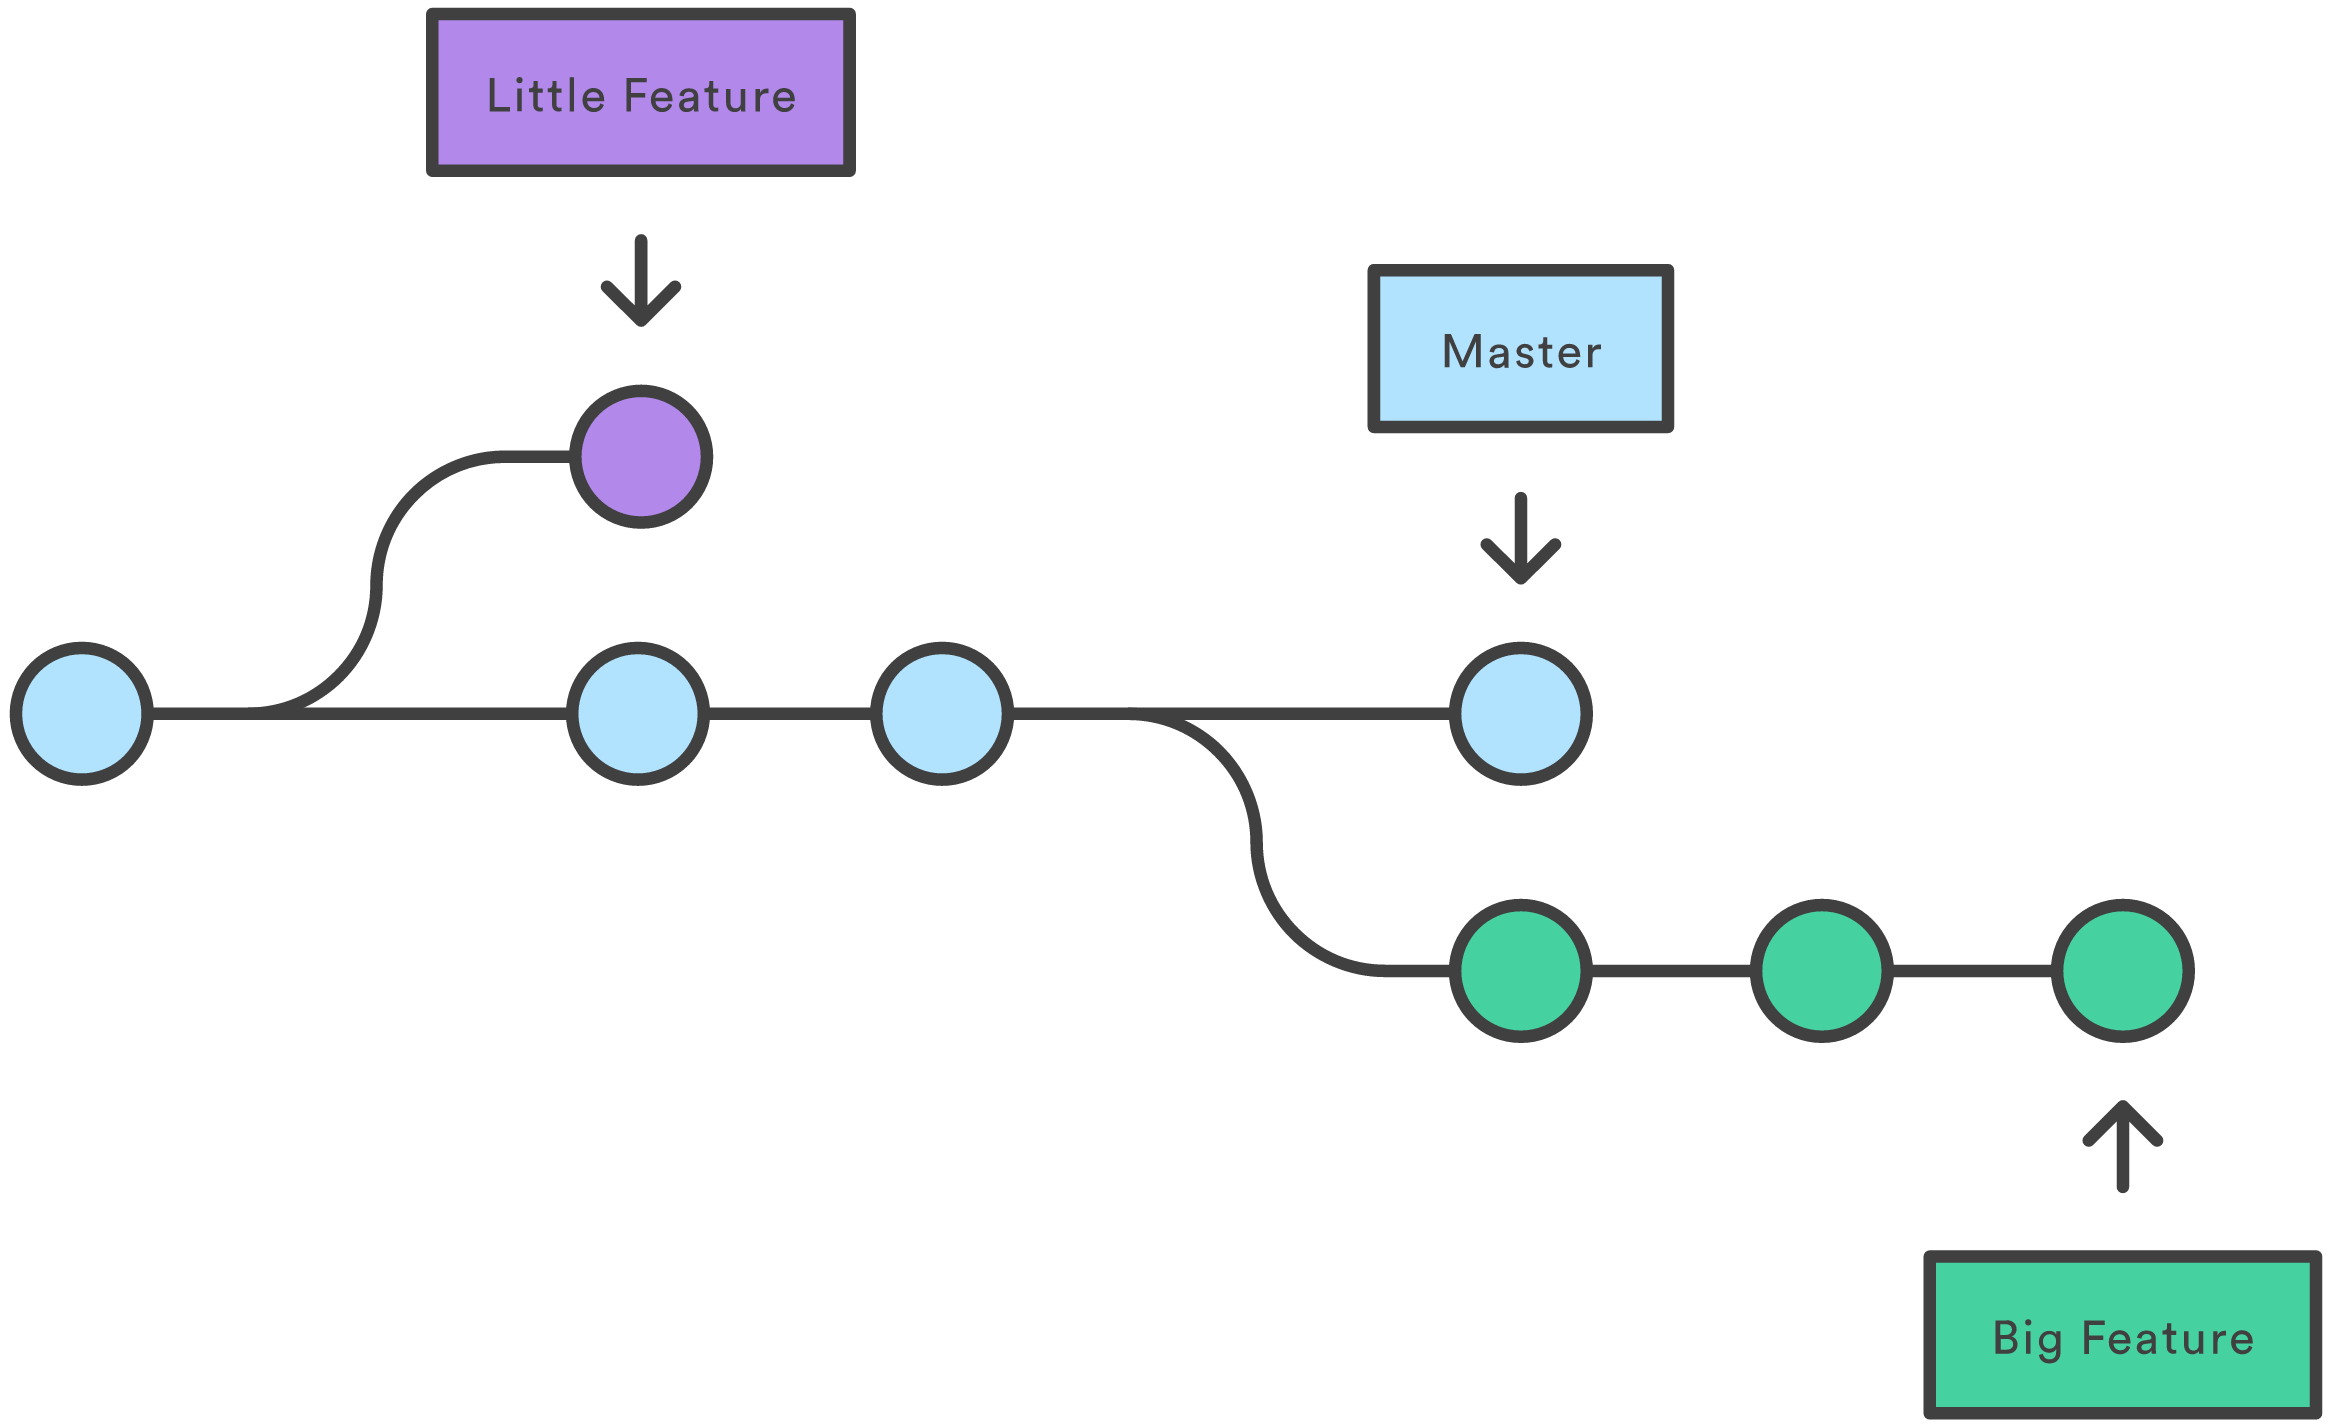
\includegraphics[width=0.9\linewidth]{images/Git-Branches-1.png}
		\caption{Visualisierung von Zweigen in Git ~\cite{GitBranches}}
	\end{center}
\end{figure}

\subsection*{Dezentralisierung}
Dadurch das jeder Benutzer sich eine lokale Kopie des Repositories samt Versionsgeschichte herunterladen kann, können die meisten Operationen ohne Internet durchgeführt werden. 

\subsection*{Sicherer Datentransfer}
Git bietet eine Vielzahl an unterschiedlichen Netzwerkprotokollen, um Daten zwischen Repositories zu übertragen. Das gängigste ist aber das sichere SSH Protokoll für Schreiboperationen und ein eigens entwickeltes Protokoll für das Fetchen und Clonen genutzt wird.

\subsection*{Sicherung der Projektgeschichte}
In Git ist es nicht möglich die Versionsgeschichte zu manipulieren. Das ist dem Hash-Wert geschuldet der bei jeder Revision (Commit) gespeichert wird. Dieser Wert basiert immer auf der vollständigen Geschichte, die bis zu jener Revision vorangegangen ist. 


\newpage
\clearpage
\section{Docker}\label{sec:Docker}
\small{\cite{docker_wiki}}{\cite{docker_glossary}}
\section*{Erläuterung}
Docker ist eine in Go geschriebene freie Software zur Erstellung von Containern um somit die Containervirtualisierung zu ermöglichen. Die Containervirtualisierung ist ein Hilfsmittel, um eigenständige und isolierte Gast-Betriebssysteme auf einem Host-Betriebssystem auszuführen. Dieses Verfahren gilt als besonders Ressourcenschonend und nützlich im Testbetrieb, da man schnell Container erstellen kann und diese auch löschen falls sie fehlerhaft sind. Ein weiterer Vorteil liegt darin, dass die Container auf den Kernel des Hauptbetriebssystems zugreifen können. Positiv anzumerken ist auch die Portierung, da lediglich die Ausführung eines sogenannten Dockerfiles ausreicht um die ganze Applikation zu starten. Docker kann mit allen gängigen Betriebssystemen wie Linux, Windows und MacOS verwendet werden. Im Nachfolgenden werden die zuvor verwendeten Begriffe erläutert.

\section*{Terminologie}
Um die Technologie und Architektur hinter Docker zu verstehen ist es wichtig einige Grundbegriffe zu wissen. Die wesentlichen werden im Folgenden näher erklärt.
\subsubsection*{Image}
Images sind schreibgeschützte Speicherabbilder von einem Container. Diese Abbilder sind portabel und können in Repositories, wie zum Beispiel das offizielle Docker-Image-Registry Docker Hub, veröffentlicht werden. Des Weiteren bestehen sie meistens aus mehreren Schichten und können in multiplen Containern gestartet werden.
\subsubsection*{Container}
Ein Container ist eine aktive Instanz eines Images und ist ausführbar, wenn ein Container keine Anwendung ausführt oder mit einem Auftrag fertig ist wird er automatisch beendet.
\subsubsection*{Dockerfile}
Ein Dockerfile ist eine Textdatei die mit diversen Kommandos ein Image beschreibt. Diese werden beim Starten nacheinander ausgeführt und für jeden Befehl ein Layer angelegt.
\newpage \subsubsection*{Docker Hub}
Docker Hub ist eine Onlineplattform für Docker-Images und Repositories. Dabei ist der Online-Dienst in einen privaten und öffentlichen Teil aufgegliedert. Im öffentlichen Teil dürfen alle Mitglieder Images hochladen und die offiziellen Images von zum Beispiel Linux Distributionen sind hier wiederzufinden. Im privaten Teil wiederum können Personen für firmeninterne Zwecke Images hochladen zu denen ausgewählte Personen Zugang haben.

\section*{Docker Architektur}
\begin{figure}[!h]
	\begin{center}
		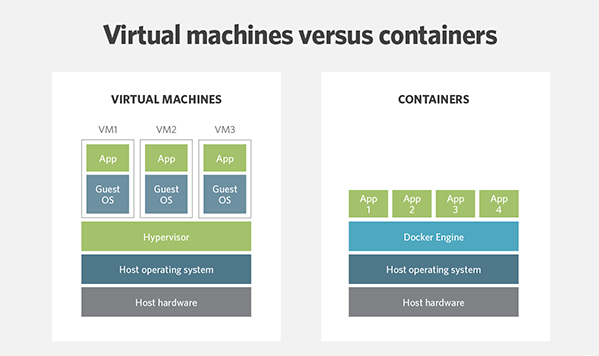
\includegraphics[width=0.7\textwidth]{images/container_vs_vm.png}
		\caption{Docker-Container sind durch ihre Architektur leichtgewichtiger als virtuelle Maschinen ~\cite{docker_101}}
	\end{center}
\end{figure}

\begin{figure}[!b]
	\begin{center}
		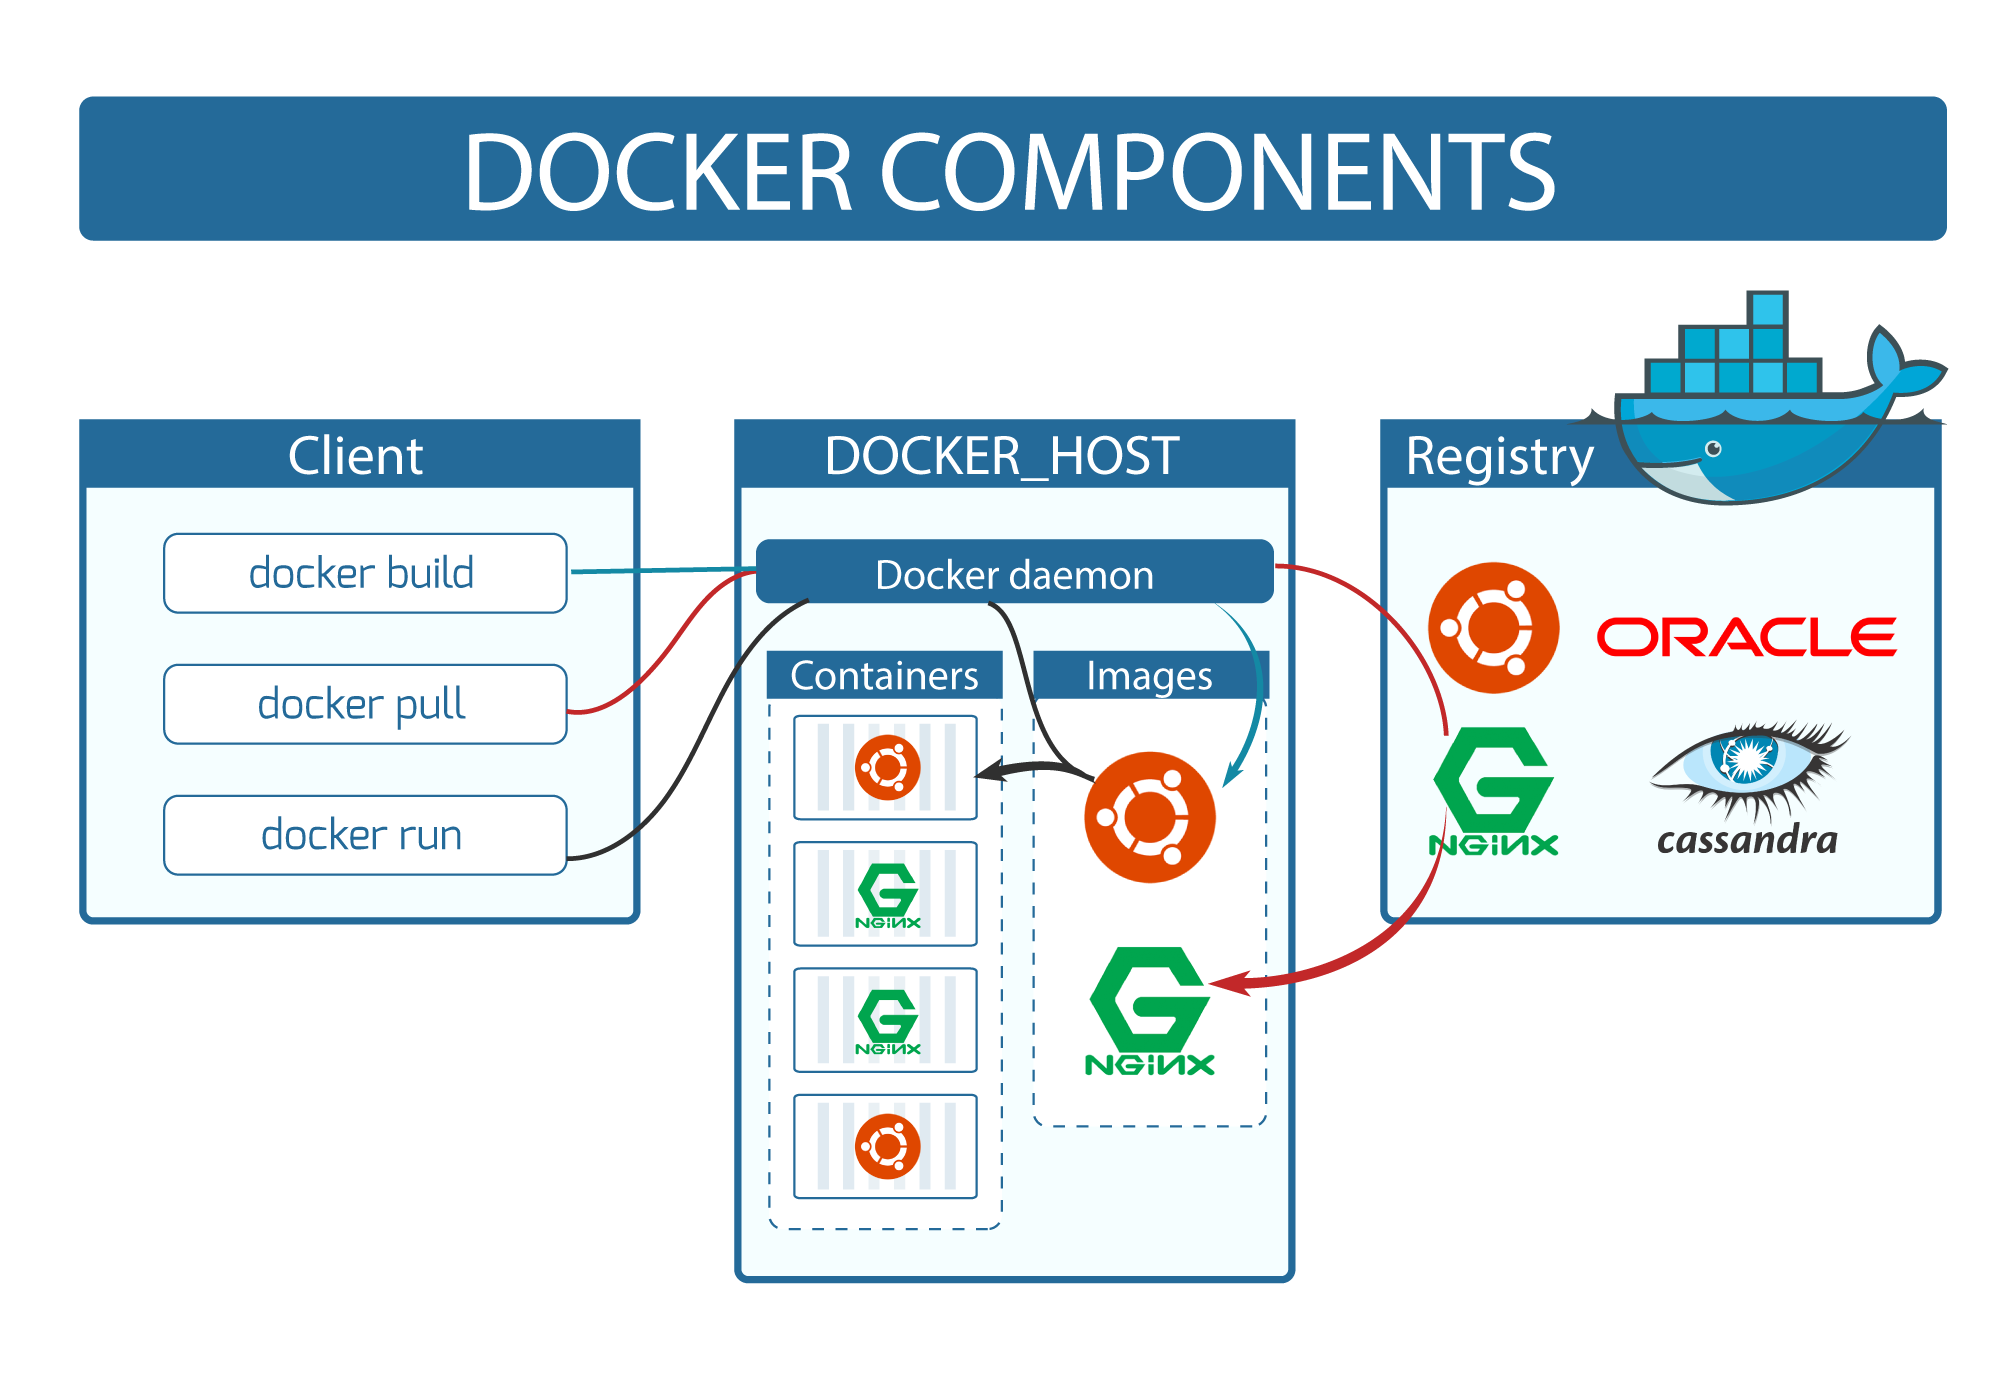
\includegraphics[width=0.7\textwidth]{images/docker_architecture.png}
		\caption{Docker Komponenten ~\cite{docker_101}}
	\end{center}
\end{figure}

\section*{Verwendung}
Der Bad-Designer bietet die Möglichkeit an in einem Docker-Container zu laufen. Dazu wurden ein \textit{docker-compose.yml} und ein \textit{Dockerfile} geschrieben die ein NGINX-Image herunterladen und die notwendigen Dateien von der Applikationen auf den NGINX-Container hochladen. Mit dem Befehl \textit{docker-compose up} wird der ganze Prozess innerhalb kürzester Zeit gestartet und mit \textit{docker-compose down} wieder, wenn benöntigt, beendet. 